\documentclass[a0,final]{a0poster}
%%%Load packages
\usepackage{tipa}
\usepackage{amsmath}
\usepackage{enumerate}
\usepackage{graphicx}
\usepackage{float}
\usepackage[scriptsize]{subfigure}
\usepackage{caption}
\usepackage{multirow}
\usepackage{color}
\usepackage{natbib}
\usepackage{ragged2e}
\usepackage{multicol} 			%3-column layout
\usepackage[left=3cm,right=3cm,bottom=0cm,top=0cm]{geometry}			%Reset margins
\usepackage{helvet}				%Load Helvetica font & CM math
\usepackage{color}				%Needed for colour boxes & coloured text
\usepackage{graphics}
\usepackage{float}
\usepackage[shortlabels]{enumitem}
\floatstyle{plaintop}
\restylefloat{figure}
\newlength{\mylen}
\setbox1=\hbox{$\bullet$}\setbox2=\hbox{\small$\bullet$}
\setlength{\mylen}{\dimexpr0.75\ht1-0.5\ht2}
\renewcommand\labelitemi{\raisebox{\mylen}{\small$\bullet$}}

%%%Define colours and lengths
\definecolor{headingcol}{rgb}{1,1,1}	%Colour of main title
\definecolor{boxcol}{rgb}{0.7,0.2,0.2}		%Edge-colour of box and top banner
\fboxsep=1cm							%Padding between box and text
\setlength{\columnsep}{1cm}				%Set spacing between columns
\renewcommand{\familydefault}{\sfdefault}	%Set main text to sans-serifb
%%%Format title
\makeatletter							%Needed to include code in main file
\renewcommand\@maketitle{%
\null									%Sets position marker
{
\vspace*{8cm}
\color{headingcol}\sffamily\Huge		%Set title font and colour
\@title \par}%
\vskip 1em%
{
\color{white}\sffamily\LARGE				%Set author font and colour
\lineskip .5em%
\begin{tabular}[t]{l}%
\@author
\end{tabular}\par}%
\vskip 1cm
\par
}
\setlength{\parskip}{0cm}
\setlength{\parindent}{1em}
\makeatother

\title{\Huge{Vowel Dynamics and Social Meaning in York, Northern England}}

\author{Daniel Lawrence\\The University of Edinburgh\\\hspace{0.5cm}daniel.lawrence@ed.ac.uk}

\begin{document}
\hspace{-4cm}								%Align with edge of page, not margin
\vspace{-2cm}

\includegraphics{Black_Landscape.pdf}

%\colorbox{boxcol}{							%Coloured banner across top
\begin{minipage}{1191mm}					%Minipage for title contents
\vspace{-18cm}
\maketitle
\end{minipage}
%}
\vspace{.5cm}

\begin{multicols*}{4}							%Use 3-column layout
			\raggedcolumns			%Don't stretch contents vertically
\section*{Introduction}
\setlist[enumerate,1]{leftmargin=2.3cm}
\begin{itemize}
 \item{As time-varying acoustic events, speech sounds offer a wide range of variable cues which could potentially attach to the social meanings available in a speech community.} 
 \item{The present study explores dynamic variation and change in the \textsc{goat} vowel (\textipa{/o/}) in York, Northern England, with a view to discovering:\vspace*{.5cm} \begin{enumerate}[(a)]\item{how dynamic properties of this vowel vary \textbf{in production}.}\vspace*{.5cm}\item{the extent to which this variation is available as a social-indexical cue \textbf{in perception.}}\end{enumerate}}
\end{itemize}
\vspace{-1cm}
\section*{Data}
\begin{itemize}
\item{52 sociolinguistic interviews (inc. interview, map task, word list) conducted in York, Northern England.}
\item{Social perception data from the same individuals.}
\end{itemize}
\vspace*{0.5cm}
\begin{table}[H]
\centering
\begin{tabular}{l|l|l}
Birth year&Female & Male \\
1935-1960 &7 &5\\
 1961-1980& 8 & 11\\
1981-2000& 10 &11\\
\end{tabular}
  \end{table}
\section*{/o/ fronting and diphthongization in York}
\begin{itemize}
\item{F1/F2/F3 Measurements taken at 20 equidistant points along the vowel trajectory.}
\item{Generalized Additive Mixed Models fit to F2 trajectories, predicting F2 as a smooth function of time.}
\item{Social factors tested: speaker year of birth, gender...}
\item{+3 composite variables derived from a factor analysis of interview responses:\begin{itemize}\item{
mobility index (-2 +2)} \item{regional identity index (-2 +2)} \item{general SES index (-2 +2)}\end{itemize}}
\end{itemize}
\begin{minipage}{0.15\textwidth}
\raggedright
\begin{figure}[H]
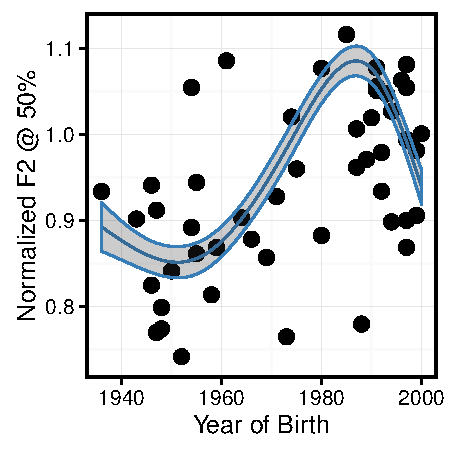
\includegraphics[scale=1.6]{o_fronting_scurve.pdf}
\caption*{\textbf{(a) Main effect of speaker year of birth}}
\end{figure}
\end{minipage}
\hspace*{-5cm}
\begin{minipage}{0.125\textwidth}
\vspace*{2cm}
\begin{itemize}
\raggedright
\item{Evidence of ongoing fronting of /o/}
\item{This change involves:\begin{itemize}\item{A rise in F2 at the offglide across speaker groups}\item{Additional fronting at the vowel midpoint among more mobile speakers, resulting in a greater curvature in the vowel trajectory}\end{itemize}}
\item{Trajectories of high/low mobility groups have become more distinct over time}
\end{itemize}
\end{minipage}
\begin{figure}[H]
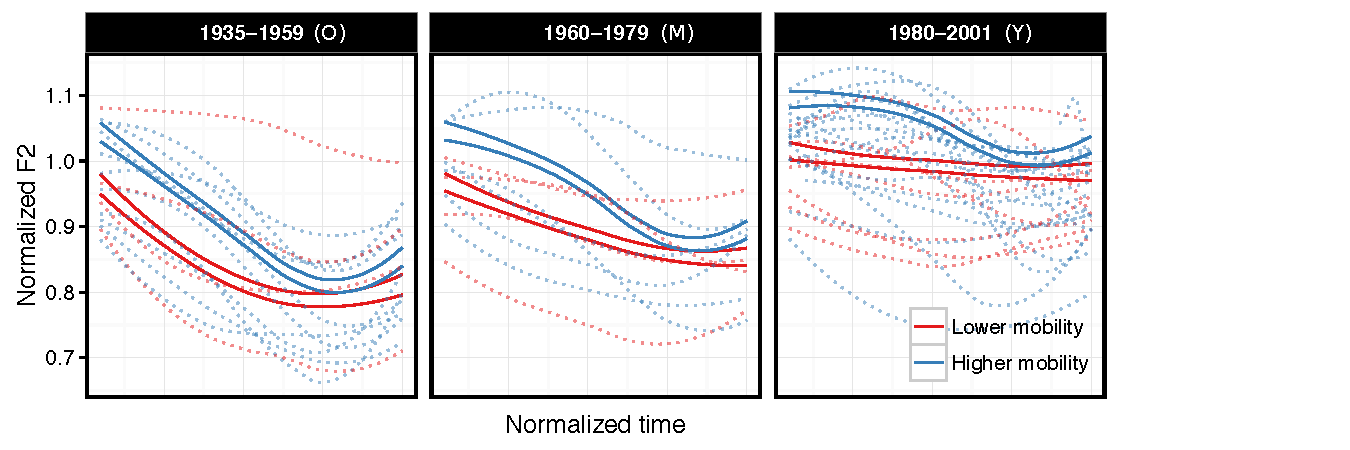
\includegraphics[scale=1.5]{o_mobility_curve.pdf}
\caption*{\hspace*{-6cm}\textbf{(b) Interaction of year of birth and mobility index}}
\end{figure}
\subsubsection*{(c) Interaction of fronting and diphthongization}
\begin{minipage}{0.13\textwidth}
\vspace*{-3cm}
\begin{figure}[H]
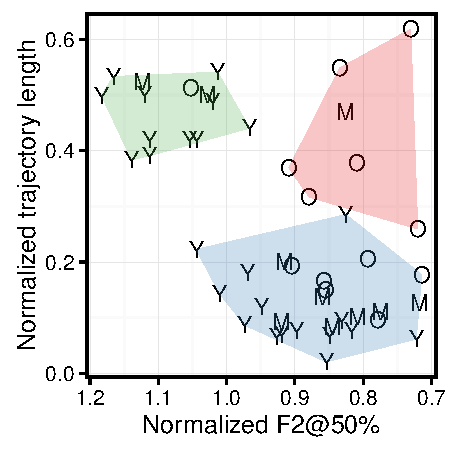
\includegraphics[scale=1.9]{o_fronting_dip.pdf}
\end{figure}
\end{minipage}
\begin{minipage}{0.12\textwidth}
\raggedright
\vspace*{.5cm}
\begin{itemize}
\item{Speakers appear to cluster into three groups:\begin{itemize}
\item{Those with back /o/ realizations, who vary in terms of their trajectory length (red)}
\item{Those with fairly back, monophthongal realizations (blue)}
\item{Those with fronted, diphthongal realizations (green)}\end{itemize}}
\item{Apparent lack of fronted monophthongs consistent with Haddican et al. (2013)}
\end{itemize}
\end{minipage}
\vspace*{-1cm}
\section*{Investigating sociolinguistic perception}
\vspace*{-.5cm}
\begin{itemize}
\item{We know that:\begin{itemize}\item{Back /o/ variants are typical of older speakers}\item{Diphthongal variants are typical of more mobile/middle-class speakers}\item{Monopthongal variants are possibly associated with regional identity (Haddican et al., 2013)}\end{itemize}}
\item{To what extent are listeners sensitive to these patterns \\ in perception?}
\end{itemize}
\vspace*{-1cm}
\begin{figure}[H]
\begin{minipage}{0.25\textwidth}
\raggedright\textit{Figure 2: \textipa{/o/} variants tested}\\
\vspace*{-0.25cm}
\centering
\footnotesize
\begin{tabular}{llllll}
&&&&&\\
                  &           & \textit{Fronting}          &             &                   &\\
                &  \multicolumn{3}{l}{$\xleftarrow{\hspace*{12cm}}$  }   &                              \\ \vspace*{-0.3cm}
\multirow{5}{*}{$\rotatebox[origin=c]{90}{$\underleftarrow{\rule{1cm}{0pt}\mathsf{\textit{Diphthongization\rule{2cm}{0pt}}}}$}$}                 &&&& &                \\
               & \LARGE{\textbf{\textipa{\o:}}}&\LARGE{\textbf{\textipa{8:}}}&\LARGE{\textbf{\textipa{o:}}}&&\\
 & Mid-front  & Mid-central   & Mid-back   &         &          \\
        &\LARGE{\textbf{\textipa{eU}}}&\LARGE{\textbf{\textipa{9U}}}&\LARGE{\textbf{\textipa{oU}}}&&\\
                   & Mid-front   & Mid-central  & Mid-back \\
                   &(fronted onset)&(centralized onset)&(diphthong)&&\\
                   &\LARGE{\textbf{\textipa{9y}}}&\LARGE{\textbf{\textipa{90}}}&&&\\
                   &Mid-front  &Mid-central  &&&\\
                   &(fronted offglide)&(centralized offglide)&&&\\
\end{tabular}
\end{minipage}
\begin{minipage}{0.23\textwidth}
\vspace*{1cm}
\normalsize
\raggedright\textit{Figure 3: Visual stimuli}\\
\vspace*{1cm}

\begin{tabular}{lllll}
\multirow{2}{*}{$\rotatebox[origin=t]{90}{$\overbrace{\rule{2cm}{0pt}\mathsf{\textit{Rural}}\rule{2cm}{0pt}}$\hspace*{-5cm}}$} &
\includegraphics[scale=0.6]{M_O_MC_L_1.png} & 
\includegraphics[scale=0.6]{M_Y_MC_L_1.png} 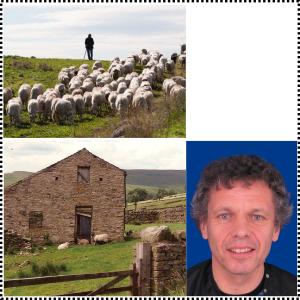
\includegraphics[scale=0.6]{M_O_WC_L_1.png} &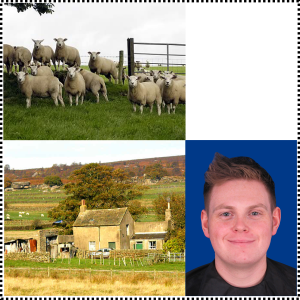
\includegraphics[scale=0.6]{M_Y_WC_L_1.png} \\ \vspace*{-1cm}
 $\rotatebox[origin=t]{90}{\hspace*{3cm}$\overbrace{\rule{2cm}{0pt}\mathsf{\textit{Urban}}\rule{2cm}{0pt}}$}$
    &
\includegraphics[scale=0.6]{M_O_MC_NL_1.png} & 
\includegraphics[scale=0.6]{M_Y_MC_NL_1.png} 
\includegraphics[scale=0.6]{M_O_WC_NL_1.png} & 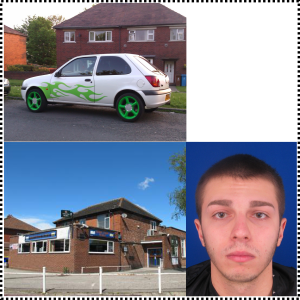
\includegraphics[scale=0.6]{M_Y_WC_NL_1.png}\\\vspace*{-3.5cm}
    &\multicolumn{4}{l}{
$\underbrace{\rule{7cm}{0pt}{\textit{Social class: Middle/Working}}\rule{5cm}{0pt}}$}\\
    &\multicolumn{4}{l}{
    $\underbrace{\rule{2cm}{0pt}{\textit{Age: Older/Younger}}\rule{2cm}{0pt}}$$\underbrace{\rule{2cm}{0pt}{\textit{Age: Older/Younger}}\rule{1cm}{0pt}}$}\\
   
\end{tabular}
\end{minipage}
\end{figure}
\vspace*{2cm}
\begin{minipage}{.23\textwidth}
\begin{itemize}
\item{\textbf{Task:} \begin{itemize}\item{Participants are told they are listening to an actor pretending to be one of a set of characters in a TV sitcom set in York.}
\item{\textbf{Training phase:} Participants sort the images according to questions e.g. `Which character comes from Rural Yorkshire'?}
\item{\textbf{Testing phase:} Participants see the characters in `minimal pairs', hear a speech token, and select the character which they think the actor is pretending to be.}\end{itemize}}
\end{itemize}
\end{minipage}
\columnbreak
\section*{Modeling sociolinguistic perception}
\begin{minipage}{0.24\textwidth}
\begin{itemize}
\item{Strategy: analyze responses for each social dimension separately -- social class (WC/MC), regional identity (Urban/Rural) age (Older/Younger).}
\item{Responses modeled using hierarchical GLMs with a logit link.}
\item{Individual-level variability modeled through listener-level intercepts and (variant|listener) random slopes.}
\item{Parameter estimates obtained through MCMC in \textit{rstanarm} (Gabry \& Goodrich, 2016). Priors were $t$-distributions with 7 degrees of freedom and a scale of 2.5.}
\end{itemize}
\end{minipage}

\section*{Results}
\begin{minipage}{0.24\textwidth}
\begin{itemize}
\item{Plots show the inverse-logit transformed posterior distribution of each parameter, representing the expected probability that each variant will cue a selection on the social dimension labeled on each plot.}
\item{Where error bars (showing 95$\%$ credible intervals) do not cross zero, there is reliable evidence that the variant impacted listeners' selections.}
\item{Where the mean of one parameter lies outside the 95$\%$ CI of another, there is evidence that the variants differed from each other in influencing listeners' responses.}
\end{itemize}
\end{minipage}
\subsubsection*{/o/ variation as an index of social class}
\vspace*{-1cm}
\begin{minipage}{0.12\textwidth}
\vspace*{-2.75cm}
\raggedright
\hspace*{-2.5cm}
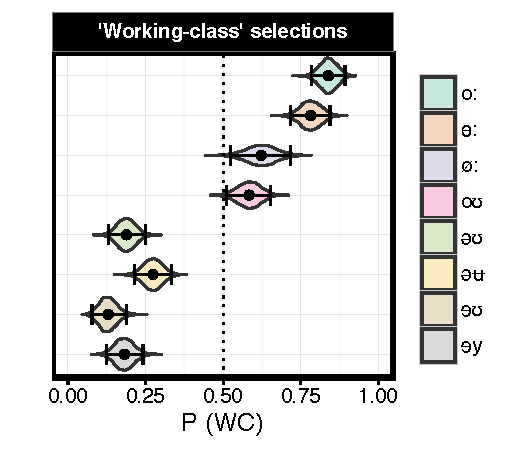
\includegraphics[scale=2.2]{ow_class_effects.pdf}
\end{minipage}
\hspace*{1.75cm}
\begin{minipage}{0.105\textwidth}
\vspace*{2cm}
\raggedright
\begin{itemize}
\item{Clear effect of diphthongization -- with the exception of the back variant \textipa{[oU]}, diphthongs tend to disfavour `WC' responses}
\item{Within monophthongs, fronting reduces the probability of a `WC' selection}
\item{Within diphthongs, fronting increases the probability of a `MC' selection, although less radically}
\item{Fronting at the offglide is marginally less `MC' than fronting at the vowel midpoint.}
\end{itemize}
\end{minipage}
\subsubsection*{/o/ variation as an index of urban/rural identity}
\begin{minipage}{0.12\textwidth}
\hspace*{-2.75cm}
\vspace*{-2.75cm}
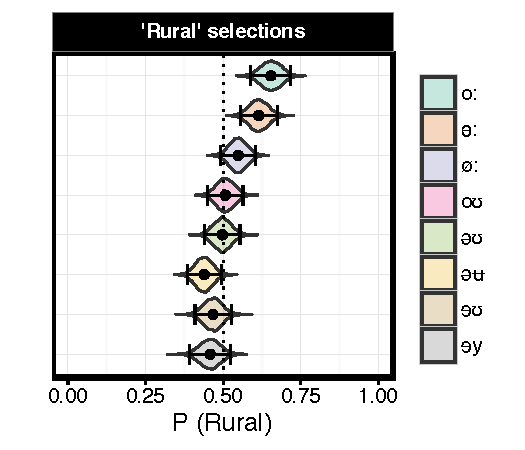
\includegraphics[scale=2.2]{ow_rural_effects.pdf}
\end{minipage}
\hspace*{1.5cm}
\begin{minipage}{0.11\textwidth}
\vspace*{-4cm}
\raggedright
\begin{itemize}
\item{Only the most back monophthongs reliably cue a `rural' selection}
\item{Fronting monophthongs reduces their potential to index `rural'}
\item{Non-back diphthongs are consistently percieved as less `rural' than monophthongs}
\end{itemize}
\end{minipage}
\subsubsection*{/o/ variation as an index of age}
\vspace*{-.5cm}
\begin{minipage}{0.13\textwidth}
\hspace*{-1.4cm}
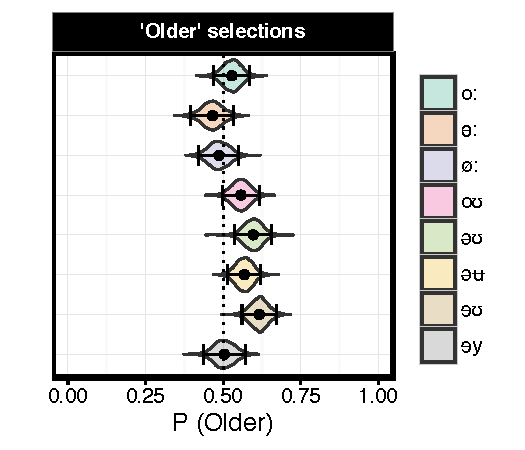
\includegraphics[scale=2.2]{ow_age_effects.pdf}
\end{minipage}
\hspace*{1.75cm}
\begin{minipage}{0.1\textwidth}
\vspace*{1cm}
\raggedright
\begin{itemize}
\item{Only fronted diphthongs are a reliable index of age}
\item{Diphthongs are more likely to cue `Older' selections than monophthongs, with the exception of the most back monophthongal variants}
\item{Within both monophthongs and diphthongs, fronting lowers the probability of an `Older' selection}
\item{Fronting at the offglide of a diphthong sounds less old than fronting at the vowel onset.}
\end{itemize}
\end{minipage}
\vspace*{-1.75cm}
\subsubsection*{Evidence of listener variability}
\vspace*{-.25cm}
\begin{minipage}{0.13\textwidth}
\hspace*{-1.4cm}
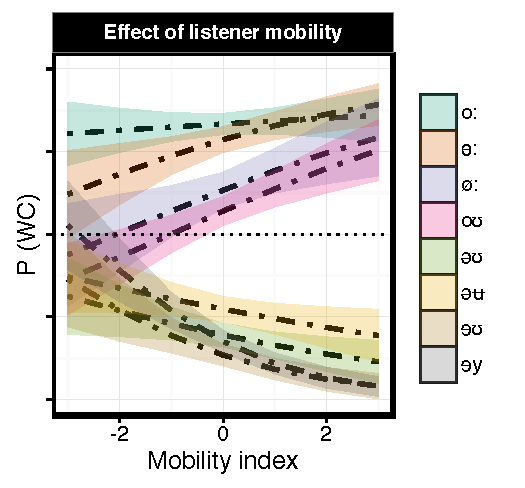
\includegraphics[scale=2.2]{o_perception_dim3_sd_main.pdf}
\end{minipage}
\hspace*{1.75cm}
\begin{minipage}{0.1\textwidth}
\vspace*{-4cm}
\raggedright
\begin{itemize}
\item{More mobile listeners are more sensitive to diphthongization as a cue to social class.}
\item{This may reflect the role of listeners' experience of regional and social variation in shaping their indexical interpretations.}
\item{Please see my other poster for similar examples!}
\end{itemize}
\end{minipage}
\vspace*{-2cm}
\section*{Conclusion}
\begin{minipage}{.25\textwidth}
\vspace*{-.5cm}
\begin{itemize}
\item{Ongoing fronting and diphthongization of \textipa{/o/} results in a range of dynamic variation.}
\item{The social interpretation of /o/ variation often reflects the distribution of that variation in production, but not always.}
\item{In some cases, listeners' perceptual inferences are consistent with production:\begin{itemize}\item{diphthongization and social class.}\item{fronting, age and social class.}\end{itemize}}
\item{In other cases, there is a mismatch between social perception and production:\begin{itemize}\item{fronted diphthongs heard as `old', but are used almost exclusively by younger speakers.}\end{itemize}}
\item{A possible interpretation: listeners' social-indexical knowledge is informed by ideologically-structured schemata (e.g. Eckert (2008); Campbell-Kibler (2009), rather than being based primarily on the social distribution of variation in the speech community (e.g. Docherty \& Foulkes, 2014). As a result, social interpretations may reflect the social patterning of variants in production, but may also contrast with them.}



\end{itemize}
\end{minipage}
\vspace*{-1.5cm}
\subsubsection*{References}
\tiny
\begin{description}

\item[Campbell-Kibler, K. (2009).]{The nature of sociolinguistic perception. Language Variation and Change, 21(01), 135-156.}

\item[Docherty, G. J., \& Foulkes, P. (2014).]{An evaluation of usage-based approaches to the modelling of sociophonetic variability. \textit{Lingua}, 142, 42-56.}

\item[Eckert, P. (2008).]{Variation and the indexical field. \textit{Journal of sociolinguistics}, 12(4), 453-476.}\vspace*{0.2cm}

\item[Gabry, J \& Goodrich, B (2016).]{rstanarm: Bayesian Applied Regression Modeling via Stan. R package version 2.9.0-4.http://CRAN.R-project.org/package=rstanarm}


\item[Haddican, B., Foulkes, P., Hughes, V., \& Richards, H. (2013).]{Interaction of social and linguistic constraints on two vowel changes in northern England. \textit{Language Variation and Change}, 25(03), 371-403.}


\end{description}
%\bibliographystyle{plain}
%\bibliography{halobib}

\end{multicols*}
\end{document}
